\section[Wykład 5: 23-III-2017]{Algebraiczna teoria grafów}
\begin{minipage}{.4\textwidth}
\begin{figure}[H]
%\begin{wrapfigure}{r}{0.3\textwidth}
\centering
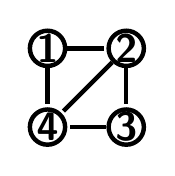
\begin{tikzpicture}[shorten >=1pt, auto, node distance=3cm, ultra thick,main node/.style={circle,draw,minimum size=.4cm,inner sep=0pt]}]%fill=black,
\begin{scope}[every node/.style={font=\sffamily\Large\bfseries}]
\node[main node] (v1) at (0,1) {1};
\node[main node] (v2) at (1,1) {2};
\node[main node] (v3) at (1,0) {3};
\node[main node] (v4) at (0,0) {4};
\end{scope}
\begin{scope}
\draw  (v1) edge node{} (v2);
\draw  (v1) edge node{} (v4);
\draw  (v2) edge node{} (v3);
\draw  (v2) edge node{} (v4);
\draw  (v3) edge node{} (v4);
%\draw  (v) edge node{} (v);
\end{scope}
\end{tikzpicture}
\caption*{Graf macierzy $A$.}
%\end{wrapfigure}
\end{figure}
\end{minipage}%
\begin{minipage}{.4\textwidth}
$$A=\begin{bmatrix}
0&1&0&1\\
1&0&1&1\\
0&1&0&1\\
1&1&1&0
\end{bmatrix}$$
\end{minipage}





\textbf{Pytanie: }Czy wektor $\begin{bmatrix}
0\\-1\\0\\1
\end{bmatrix}$ jest wektorem własnym  macierzy $A$?

\begin{enumerate}[label=\Roman*.]
\item Wymnożyć:
$$\begin{bmatrix}
0&1&0&1\\
1&0&1&1\\
0&1&0&1\\
1&1&1&0
\end{bmatrix}\begin{bmatrix}
0\\-1\\0\\1
\end{bmatrix}=\begin{bmatrix}
0\\1\\0\\-1
\end{bmatrix}=-1\begin{bmatrix}
0\\-1\\0\\1
\end{bmatrix}$$

\item Przyporządkowywanie wartości wektora własnego do poszczególnych wierzchołków grafu. 
\end{enumerate}

\subsection{Laplasjan}
\begin{definition}[Laplasjan]
Laplasjanem grafu $G=(V,E)$ o $n$ wierzchołkach nazywamy macierz $n\times n$ oznaczoną $$L(G)=[l_{i,j}]$$ zdefiniowaną jako: $$l_{i.j}=\left\{\begin{matrix}
\deg (i) & i=j\\
-1 & \{i,j\}\in E\\
0 & \text{ w pozostałych przypadkach}
\end{matrix}\right.$$
\end{definition}

\begin{minipage}{.3\textwidth}
\begin{figure}[H]
%\begin{wrapfigure}{r}{0.3\textwidth}
\centering
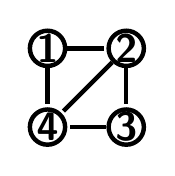
\begin{tikzpicture}[shorten >=1pt, auto, node distance=3cm, ultra thick,main node/.style={circle,draw,minimum size=.4cm,inner sep=0pt]}]%fill=black,
\begin{scope}[every node/.style={font=\sffamily\Large\bfseries}]
\node[main node] (v1) at (0,1) {1};
\node[main node] (v2) at (1,1) {2};
\node[main node] (v3) at (1,0) {3};
\node[main node] (v4) at (0,0) {4};
\end{scope}
\begin{scope}
\draw  (v1) edge node{} (v2);
\draw  (v1) edge node{} (v4);
\draw  (v2) edge node{} (v3);
\draw  (v2) edge node{} (v4);
\draw  (v3) edge node{} (v4);
%\draw  (v) edge node{} (v);
\end{scope}
\end{tikzpicture}
\caption*{Graf macierzy $A$.}
%\end{wrapfigure}
\end{figure}
\end{minipage}%
\begin{minipage}{.7\textwidth}
$$A=\begin{bmatrix}
0&1&0&1\\
1&0&1&1\\
0&1&0&1\\
1&1&1&0
\end{bmatrix} \Leftrightarrow L = \begin{bmatrix}
2&-1&0&-1\\
-1&3&-1&-1\\
0&-1&2&-1\\
-1&-1&-1&3
\end{bmatrix}$$
\end{minipage}

\begin{fact}
Jeśli graf $G$ jest $d$-regularny to: $$L=dI-A$$
\end{fact}
\noindent
Niech $G$ będzie $d$-regularny\\
Niech $\bar{v}$ będzie wektorem własnym macierzy $\bar{\bar{A}}$ o wartości własnej $\lambda$
Wtedy: 
$$\bar{\bar{L}}\bar{v}=(d\bar{\bar{I}}-\bar{\bar{A}})\bar{v}=d\bar{\bar{I}}\bar{v}-\bar{\bar{A}}\bar{v}=d\bar{v}-\lambda \bar{v}=(d-\lambda )\bar{v}$$

\begin{fact}
Jeśli $G$ o $n$ wierzchołkach jest $d$-regularny to $A$ i $L$ mają te same wektory własne, a każdej wartości własnej $\lambda $ macierzy $A$ odpowiada wartość własna $d-\lambda $ macierzy $L$
$$\textsc{Tr}[A]=\sum _{i=1}^n\lambda _i = 0$$
\end{fact}

\begin{fact}
Wszystkie wartości własne $L$ są nieujemne (\textit{$L$ jest pół-dodatnio określona})
\end{fact}

Dla grafu $d$-regularnego
$$A=\begin{bmatrix}
0&1&\cdots &1\\
1&0&\cdots &1\\
\vdots &\vdots & \ddots & \vdots \\
1&1&\cdots & 0
\end{bmatrix}\begin{bmatrix}
1\\1\\\vdots \\ 1
\end{bmatrix}=\begin{bmatrix}
\deg (v_1) \\\deg (v_2) \\\vdots \\\deg (v_n)
\end{bmatrix}=d\begin{bmatrix}
1\\1\\\vdots \\ 1
\end{bmatrix}$$


\begin{minipage}{.3\textwidth}
\begin{figure}[H]
%\begin{wrapfigure}{r}{0.3\textwidth}
\centering
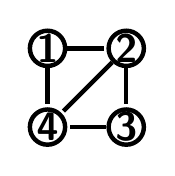
\begin{tikzpicture}[shorten >=1pt, auto, node distance=3cm, ultra thick,main node/.style={circle,draw,minimum size=.4cm,inner sep=0pt]}]%fill=black,
\begin{scope}[every node/.style={font=\sffamily\Large\bfseries}]
\node[main node] (v1) at (0,1) {1};
\node[main node] (v2) at (1,1) {2};
\node[main node] (v3) at (1,0) {3};
\node[main node] (v4) at (0,0) {4};
\end{scope}
\begin{scope}
\draw  (v1) edge node{} (v2);
\draw  (v1) edge node{} (v4);
\draw  (v2) edge node{} (v3);
\draw  (v2) edge node{} (v4);
\draw  (v3) edge node{} (v4);
%\draw  (v) edge node{} (v);
\end{scope}
\end{tikzpicture}
\caption*{Graf macierzy $A$.}
%\end{wrapfigure}
\end{figure}
\end{minipage}%
\begin{minipage}{.7\textwidth}
$$\begin{bmatrix}
2&-1&0&-1\\
-1&3&-1&-1\\
0&-1&2&-1\\
-1&-1&-1&3
\end{bmatrix}\begin{bmatrix}
1\\1\\1\\1
\end{bmatrix}=\begin{bmatrix}
0\\0\\0\\0
\end{bmatrix}$$
\end{minipage}
$d$ jest wartością własną, natomiast $0$ jest najmniejszą wartością własną każdego Laplasjanu $L$, jednocześnie najmniejszą wartością wierszy i kolumn $L$ sumują się do $0$

\begin{problem*}[$\mathsf{MAX CUT}$]
\textbf{Pytanie: } co można odczytać z wartości własnych Laplasjanów $\mu _n \geq \mu _{n-1}\geq ..\geq \mu _1 \geq 0$?

Zastosowanie - oszacowanie $\mathsf{MAX CUT}$ \newline
Mając dany graf znajdź podział jego wierzchołków na dwie części który maksymalizuje liczbę krawędzi między nimi.\\ Ta liczba to rozwiązanie problemu $\mathtt{MAX CUT}$
$$\mathtt{MAX CUT}=\max _{v_1, v_2}\{E(v_1,v_2)\}$$
\end{problem*}
\begin{theorem}
$$\mathtt{MAX CUT}\leq \frac{\mu _n*n}{4}$$ gdzie $\mu _n$ jest największą wartością Laplasjanu $L$\\
w szczególności, gdy $G$ jest $d$-regularny
$$ \mathtt{MAX CUT}\leq \frac{nd}{4}-\frac{\lambda n}{4}$$ gdzie $\lambda _n$ jest najmniejszą wartością własną macierzy $A$
\end{theorem}

\begin{remark}
Dla $K_n$
\begin{itemize}[label=$\rightarrow$]
\item wartości własne $A:\ n-1, \underbrace{-1,...,-1}_{n-1}$
\item wartości własne $L:\ 0, \underbrace{n,..n}_{n-1}$
\end{itemize}
$$\mathtt{MAX CUT}(K_n)\leq \frac{n^2}{4}$$
\end{remark}

\begin{example*}[Znaleźć wartości własne grafu $G$] Dane:\newline
\begin{minipage}{.3\textwidth}
\begin{figure}[H]
%\begin{wrapfigure}{r}{0.3\textwidth}
\centering
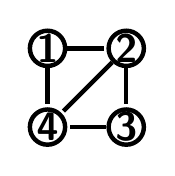
\begin{tikzpicture}[shorten >=1pt, auto, node distance=3cm, ultra thick,main node/.style={circle,draw,minimum size=.4cm,inner sep=0pt]}]%fill=black,
\begin{scope}[every node/.style={font=\sffamily\Large\bfseries}]
\node[main node] (v1) at (0,1) {1};
\node[main node] (v2) at (1,1) {2};
\node[main node] (v3) at (1,0) {3};
\node[main node] (v4) at (0,0) {4};
\end{scope}
\begin{scope}
\draw  (v1) edge node{} (v2);
\draw  (v1) edge node{} (v4);
\draw  (v2) edge node{} (v3);
\draw  (v2) edge node{} (v4);
\draw  (v3) edge node{} (v4);
%\draw  (v) edge node{} (v);
\end{scope}
\end{tikzpicture}
\caption*{Graf $G$.}
%\end{wrapfigure}
\end{figure}
\end{minipage}%
\begin{minipage}{.7\textwidth}
$$\begin{bmatrix}
2&-1&0&-1\\
-1&3&-1&-1\\
0&-1&2&-1\\
-1&-1&-1&3
\end{bmatrix}$$
\end{minipage}
\end{example*}

\begin{definition}[Liczba drzew rozpiętych grafu $G$]
$$\tau (G)$$
to liczba pod-grafów $G$ nie zawierających cykli i zawierających $n-1$ krawędzi.

Ile wynosi:
\begin{itemize}
\item $\tau (C_n)=n$
\item $\tau (P_n)=1$\footnote{To jest ścieżka} 
\item $\tau (K_n)=n^{n-2}$ Wzór Kajleja $\tau (K_n)=\frac{1}{n}n^{n-1}=n^{n-2}$
\item $\tau (G)=\binom{5}{2}-2=8$ (graf z przykładu wyżej
\end{itemize}
\end{definition}

\begin{theorem}[Kronecker]
Chcąc wyliczyć $E(G)$ weź Laplasjan $L$, skreśl jedną kolumnę i jeden wiersz (dowolny), oblicz wyznacznik powstałej macierzy (minora $L$) i ewentualnie weź jej wartość bezwzględną.
\end{theorem}
\begin{theorem}
Niech $$\mu _n \geq \mu _{n-1} \geq ... \geq \mu _2\geq \mu _1$$ będą wartościami własnymi $T$ wtedy: $$\tau (G)=\frac{1}{n}\mu _n * \mu_{n-1} * ... * \mu _2$$
\end{theorem}
\begin{figure}[H]
%\begin{wrapfigure}{r}{0.3\textwidth}
\centering
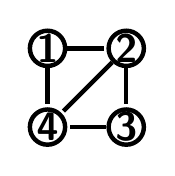
\begin{tikzpicture}[shorten >=1pt, auto, node distance=3cm, ultra thick,main node/.style={circle,draw,minimum size=.4cm,inner sep=0pt]}]%fill=black,
\begin{scope}[every node/.style={font=\sffamily\Large\bfseries}]
\node[main node] (v1) at (0,1) {1};
\node[main node] (v2) at (1,1) {2};
\node[main node] (v3) at (1,0) {3};
\node[main node] (v4) at (0,0) {4};
\end{scope}
\begin{scope}
\draw  (v1) edge node{} (v2);
\draw  (v1) edge node{} (v4);
\draw  (v2) edge node{} (v3);
\draw  (v2) edge node{} (v4);
\draw  (v3) edge node{} (v4);
%\draw  (v) edge node{} (v);
\end{scope}
\end{tikzpicture}
\caption*{Graf $G$.}
%\end{wrapfigure}
\end{figure}

\begin{align*}
\left[
\begin{array}{ccc>{\columncolor{red!20}}c}
2&-1&0&-1\\
-1&3&-1&-1\\
0&-1&2&-1\\\rowcolor{red!20}
-1&-1&-1&3
\end{array}
\right] \rightarrow \begin{vmatrix}
2&-1&0\\-1&3&-1\\0&-1&2
\end{vmatrix} = 12-2-2=8\\
\tau (G) = \frac{1}{4}4*4*2=8
\end{align*}

$$A=V\Lambda V^{-1}=V\Lambda V^T$$
$V\rightarrow $ kolumny są wektorami własnymi
\begin{align*}
\Lambda = \begin{bmatrix}
\lambda _1 & 0 & \dots & 0\\
0 & \lambda _2 & \dots & 0 \\
\vdots & \vdots & \ddots & \vdots \\
0 & 0 & \dots & \lambda _n
\end{bmatrix} & \Lambda ^m =\begin{bmatrix}
\lambda _1^m & 0 & \dots & 0\\
0 & \lambda _2^m & \dots & 0 \\
\vdots & \vdots & \ddots & \vdots \\
0 & 0 & \dots & \lambda _n^m
\end{bmatrix}
\end{align*}

%--------------------------------------------------